\documentclass[tikz]{standalone}
\usetikzlibrary{arrows, positioning}
\usetikzlibrary {arrows.meta}
\usepackage{xcolor}
\definecolor{allcolor}{RGB}{148,182,233}
\newcommand*{\equal}{=}
\begin{document}
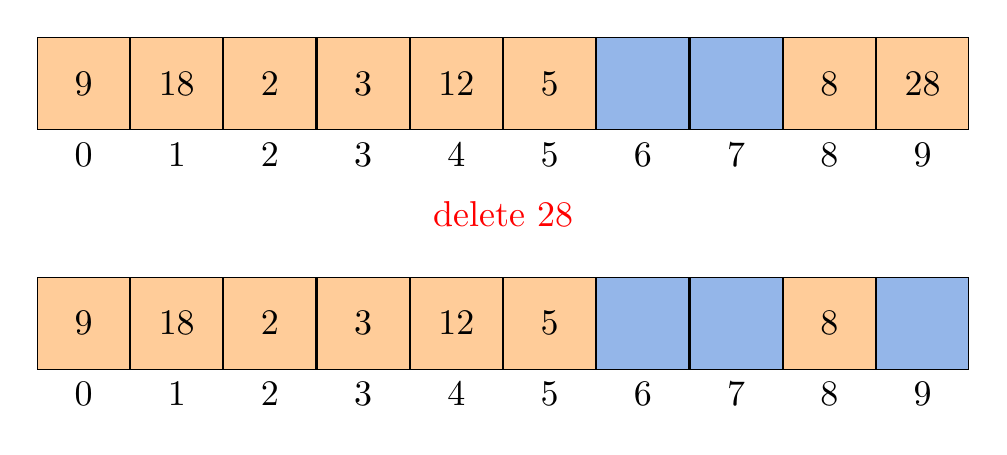
\begin{tikzpicture}[every node/.style={scale=1.3}, dot/.style={minimum size=0.1mm, circle, fill=black!90}, slot/.style={minimum size=0.9cm, rectangle}, noslot/.style={slot, fill=allcolor},
    yesslot/.style={slot, fill=orange!40}, data/.style={minimum size=0.7cm, fill=orange!40}, >=Stealth]
    \tikzstyle{textbf} = [text width=5cm,text centered]

    \matrix [row sep=1cm,nodes=draw] (table1)
    {
      \node[yesslot, label=below:$0$] {9}; &
      \node[yesslot, label=below:$1$] {18}; &
      \node[yesslot, label=below:$2$] {2}; &
      \node[yesslot, label=below:$3$] {3}; &
      \node[yesslot, label=below:$4$] {12}; &
      \node[yesslot, label=below:$5$] {5}; &
      \node[noslot, label=below:$6$] {}; &
      \node[noslot, label=below:$7$] {}; &
      \node[yesslot, label=below:$8$] {8}; &
      \node[yesslot, label=below:$9$] {28}; &
      \\
    }; 

    \matrix [row sep=1cm,nodes=draw, below=of table1] (table0)
    {
      \node[yesslot, label=below:$0$] {9}; &
      \node[yesslot, label=below:$1$] {18}; &
      \node[yesslot, label=below:$2$] {2}; &
      \node[yesslot, label=below:$3$] {3}; &
      \node[yesslot, label=below:$4$] {12}; &
      \node[yesslot, label=below:$5$] {5}; &
      \node[noslot, label=below:$6$] {}; &
      \node[noslot, label=below:$7$] {}; &
      \node[yesslot, label=below:$8$] {8}; &
      \node[noslot, label=below:$9$] {}; &
      \\
    }; 

    \node [above=of table0, red, yshift=-0.5cm] {delete $28$};

\end{tikzpicture}
\end{document}